\section{PA1: Symbolic Execution of Neural Networks}\label{sec:pa1}

In this PA you will implement an neural network (NN) verifier using symbolic execution (SE) as described in~\autoref{sec:se-smt}. You can consider NNs as a specific type of programs and thus can ``execute'' it.  SE runs the NN on symbolic inputs and returns symbolic outputs, i.e., a constraint representation.  You will represent the symbolic outputs as a logical formula and use a constraint solver to check \emph{assertions}, i.e., properties about the DNN. This PA has two parts: (1) implement SE on a given DNN, and (2) evaluate the scalability of your SE on various DNNs.

You will use Python and the Z3 SMT solver (\autoref{sec:z3}) for this assignment. \textbf{Do not} use external libraries or any extra tools (other than \texttt{z3-solver}).

\subsection{Part1: Symbolic Execution}

Consider the following fully-connected DNN with 2 inputs, 2 hidden layers, and 2 outputs.

\begin{center}
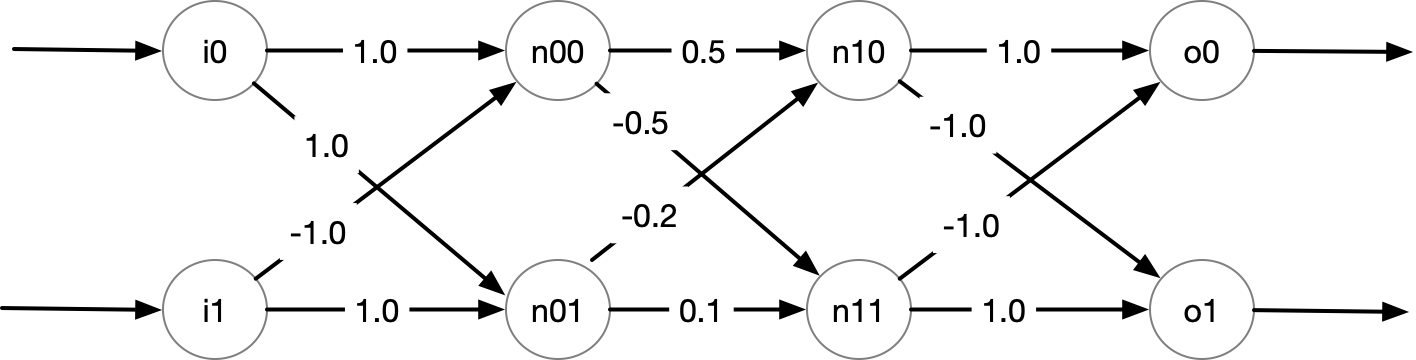
\includegraphics[width=0.8\textwidth]{figure/dnn1.png}
\end{center}

\begin{enumerate}[label=\arabic*.]
\item \textbf{DNN Encoding}: We can encode this DNN using Python:

\begin{lstlisting}[language=Python]
# (weights, bias, use activation function relu or not)
n00 = ([1.0, -1.0], 0.0, True)
n01 = ([1.0, 1.0], 0.0, True)
hidden_layer0 = [n00,n01]

n10 = ([0.5, -0.2], 0.0, True)
n11 = ([-0.5, 0.1], 0.0, True)
hidden_layer1 = [n10, n11]

# don't use relu for outputs
o0 = ([1.0, -1.0], 0.0, False)  
o1 = ([-1.0, 1.0], 0.0, False)
output_layer = [o0, o1]

dnn = [hidden_layer0, hidden_layer1, output_layer]
\end{lstlisting}

In this DNN, the outputs of the neurons in the hidden layers (prefixed with \texttt{n}) are applied with the \texttt{relu} activation function, but the outputs of the DNN (prefixed with \texttt{o}) are not.  These settings are controlled by the \texttt{True}, \texttt{False} parameters as shown above.  Also, this example does not use \texttt{bias}, i.e., bias values are all 0.0's as shown. 

Note that all of these settings are parameterized and I deliberately use this example to show these how these parameters are used (e.g., \texttt{relu} only applies to hidden neurons, but not outputs).

\item \textbf{Symbolic States}: After performing symbolic execution on \texttt{dnn}, we obtain symbolic states, represented by a logical formula relating input and output variables.

\begin{lstlisting}[language=Python]
# my_symbolic_execution is something you implement,
# it returns a single (but large) formula representing the symbolic states.
symbolic_states = my_symbolic_execution(dnn)
...
``done, obtained symbolic states for DNN in 0.1s``
assert z3.is_expr(symbolic_states)  #symbolic_states is a Z3 expression

# your symbolic states should look something like this
print(symbolic_states)   
# And(n0_0 == If(i0 + -1*i1 <= 0, 0, i0 + -1*i1),
#     n0_1 == If(i0 + i1 <= 0, 0, i0 + i1),
#     n1_0 ==
#     If(1/2*n0_0 + -1/5*n0_1 <= 0, 0, 1/2*n0_0 + -1/5*n0_1),
#     n1_1 ==
#     If(-1/2*n0_0 + 1/10*n0_1 <= 0, 0, -1/2*n0_0 + 1/10*n0_1),
#     o0 == n1_0 + -1*n1_1,
#     o1 == -1*n1_0 + n1_1)
\end{lstlisting}

\item \textbf{Constraint Solving}: We will use \texttt{Z3} to query various things about this DNN from the obtained symbolic states. Examples include:

\begin{enumerate}[label=(\alph*)]
\item Generating random inputs and obtain outputs.  Note that these are random values (that satisfy the symbolic states), so your results might look different.

\begin{lstlisting}[language=Python]
z3.solve(symbolic_states)
[n0_1 = 15/2,
    o1 = 1/2,
    o0 = -1/2,
    i1 = 7/2,
    n1_1 = 1/2,
    n1_0 = 0,
    i0 = 4,
    n0_0 = 1/2]
\end{lstlisting}

\item Simulating a concrete execution. 

\begin{lstlisting}[language=Python]
i0, i1, n0_0, n0_1, o0, o1 = z3.Reals("i0 i1 n0_0 n0_1 o0 o1")

# finding outputs when inputs are fixed [i0 == 1, i1 == -1]
g = z3.And([i0 == 1.0, i1 == -1.0])
z3.solve(z3.And(symbolic_states, g))  # you should get o0, o1 = 1, -1
[n0_1 = 0,
o1 = -1,
o0 = 1,
i1 = -1,
n1_1 = 0,
n1_0 = 1,
i0 = 1,
n0_0 = 2]
\end{lstlisting}

\item Checking assertions, i.e., verifying/proving properties about the DNN or disproving/finding counterexamples

\begin{lstlisting}[language=Python]
print("Prove that if (n0_0 > 0.0 and n0_1 <= 0.0) then o0 > o1")
g = z3.Implies(z3.And([n0_0 > 0.0, n0_1 <= 0.0]), o0 > o1)
print(g)  #  Implies (And(n0_0 > 0, n0_1 <= 0), o0 > o1)
z3.prove(z3.Implies(symbolic_states, g))  # proved

print("Prove that when (i0 - i1 > 0 and i0 + i1 <= 0), then o0 > o1")
g = z3.Implies(z3.And([i0 - i1 > 0.0, i0 + i1 <= 0.0]), o0 > o1)
print(g)  # Implies(And(i0 - i1 > 0, i0 + i1 <= 0), o0 > o1)
z3.prove(z3.Implies(symbolic_states, g))
# proved

print("Disprove that when i0 - i1 >0, then o0 > o1")
g = z3.Implies(i0 - i1 > 0.0, o0 > o1)
print(g)  # Implies(And(i0 - i1 > 0, i0 + i1 <= 0), o0 > o1)
z3.prove(z3.Implies(symbolic_states, g))
# counterexample  (you might get different counterexamples)
# [n0_1 = 15/2,
# i1 = 7/2,
# o0 = -1/2,
# o1 = 1/2,
# n1_0 = 0,
# i0 = 4,
# n1_1 = 1/2,
# n0_0 = 1/2]
\end{lstlisting}
\end{enumerate}
\end{enumerate}

\subsection{TIPS}

\begin{enumerate}[label=\arabic*.]
\item It is strongly recommend that you do symbolic execution on this DNN example \textbf{by hand} first before attempt any coding.  This example is small enough that you can work out step by step.  For example, you can do these two steps
    \begin{enumerate}[label=(\alph*)]
    \item First, obtain the symbolic states by hand (e.g., on a paper) for the given DNN
    \item Then, put what you have in code but also for the given DNN. Use Z3 format (e.g.,  you would declare the inputs as symbolic values \texttt{i0 = z3.Real("i0")}, then compute the neurons and outputs, etc)
    \item Finally, convert what you have into a general program that would work for any DNN inputs.
    \end{enumerate}

\item You can use the below method to construct Z3 formula for ReLU

\begin{lstlisting}[language=Python]
@classmethod
def relu(cls, v):
   return z3.If(0.0 >= v, 0.0, v)
\end{lstlisting}

\item Two ways of doing symbolic execution to obtain symbolic states
    \begin{enumerate}[label=(\alph*)]
    \item You can follow the traditional SE method which produces the symbolic execution trees in which each condition representing ReLU forks into two paths.  You can decide whether to do a depth-first search or breadth-first search here (they will have the same results). At the end, the symbolic states are a disjunction of the path conditions (i.e., \texttt{z3.And[path\_conds]}).
    \item But since we are using Z3, a much much simpler way, is to encode all those forked paths directly as a formula.  For example

\begin{lstlisting}[language=Python]
   if (x + y > 0):
      r = 3
   else:
      r = 4
\end{lstlisting}

Using traditional SE, you would have 2 paths,  e.g., path 1: \texttt{x+y > 0 \&\& r = 3} and path 2 : \texttt{x+y <= 0 \&\& r ==4}, from which you take the disjunction and get \texttt{(x+y > 0 \&\& r == 3) || (x+y <= 0 \&\& r ==4)}.  But for this assignment, instead of having to fork into two paths, you can use Z3 to encode both branches using the \texttt{If} function, e.g., \texttt{If(x+y>0, r==3, r==4)}  or \texttt{r==If(x+y>0,3,4)}.  The results of these two methods are exactly the same at the end, just that the prior, traditional one you do more work while the later you do less.  It is up to you.
    \end{enumerate}

\item When \texttt{bias} is none-zero, then it will simply be added to the neuron computation, i.e., \texttt{neuron =  relu(sum(value\_i * weight\_i) + bias)}.  For example, if \texttt{bias} is \texttt{0.123}  then for neuron \texttt{n0\_0} we would obtain \texttt{n0\_0 == If(i0 + -1*i1 + 0.123 <= 0, 0, i0 + -1*i1 + 0.123)}.



% \item Z3 Resources

% Some links for Z3 that you might find useful
% \begin{itemize}
%     \item \url{https://microsoft.github.io/z3guide/programming/Z3%20Python%20-%20Readonly/Introduction} : good intro for beginner.
%     \item \url{https://z3prover.github.io/api/html/namespacez3py.html} : Z3 API document
% \end{itemize}

% However, you don't really need to know much about Z3 except for a few methods used in class and given throughout this PA.  Here's probably all you need to know

% \begin{lstlisting}[language=Python]
% import z3 

% x = z3.Real("x")
% y = z3.Real("y")
% f0 = x == 3.5  # an equality x == 3.5
% f1= x == y + 3.5  # an equality x = y + 3.5
% f2 = z3.If(y <= 0, 0, y)   

% f3 = z3.Implies(x <= 3.7, x <= 5)  #x <= 3.7 => x <= 5
% z3.prove(f3)  #can prove

% f4 = z3.Implies(x<=5, x<=3.7)
% z3.prove(f4)   # cannot prove

% mylist = [x <= 3,   y <= 5]
% f5 = z3.And(mylist)
% z3.solve(f5)  #check if f5 is satisfiable,  should be yes 
% \end{lstlisting}

\item Using \texttt{Tensorflow Keras} (or \texttt{Pytorch})

In my example above, I create a DNN using simple Python lists.  But you can also use \texttt{Tensorflow Keras} (or \texttt{Pytorch}) to create a DNN.  It might be simpler that way as then you can reuse existing methods from these Python packages.  You will still need to implement symbolic execution, just that instead the input DNN being Python lists, they are now Tensorflow or Pytorch.  Also note that if you use \texttt{tensorflow} or \texttt{pytorch}, then be sure to indicate what packages are needed to run your program in the \textbf{README} file, i.e., \texttt{pip install ...}.

Below is the tensorflow representation of the DNN example above. 

\begin{lstlisting}[language=Python]
import tensorflow as tf
from tensorflow import keras
from tensorflow.keras.models import Sequential
from tensorflow.keras.layers import Dense
from tensorflow.keras import activations

model = Sequential()

# layer 0: nodes n00, n01
model.add(Dense(units=2,
                input_shape=(2, ),    # 2 inputs (i.e., i0, i1 in the Figure)
                activation=activations.relu,  # relu activation
                kernel_initializer=tf.constant_initializer(
                    [[1.0, 1.0],  # weights of n00
                    [-1.0, 1.0]  # weights of n01
                    ]),
                bias_initializer=tf.constant_initializer(
                    [[0.0],  # bias of n00
                    [0.0]]  # bias of n01
                ), 
                dtype='float64'
                ))

# layer 1: nodes n10, n11
model.add(Dense(units=2,
                activation=activations.relu,
                kernel_initializer=tf.constant_initializer(
                    [[0.5, -0.5], [-0.2, 0.1]]),
                bias_initializer=tf.constant_initializer([[0.0], [0.0]]),
                dtype='float64'
                ))

# last layer: nodes represent outputs o0, o1
model.add(Dense(units=2,
                activation=None,  # no activation function for output nodes
                kernel_initializer=tf.constant_initializer(
                    [[1.0, -1.0], [-1.0, 1.0]]), # weights of o0, o1
                bias_initializer=tf.constant_initializer([[0.0], [0.0]]),  # bias of o0, o1
                dtype='float64'
                ))
\end{lstlisting}
\end{enumerate}

\subsection{Part:2: Evaluation}
In this part you will show that symbolic execution \emph{does not} scale on large DNNs.

\begin{enumerate}
    \item You will create a function \texttt{create\_random} that takes as input a list of positive integers representing the sizes of the neurons \texttt{[\#inputs, \#ofnumbers, \#ofneurons, ..., \#outputs]}, and create a neural network of that size with \emph{random} weights and bias (e.g., between say $-5$ and $5$).
    \item You will run symbolic execution on this network as you did in PA1, get its results, and time the solving process.
    \item You will do this for various sizes of neurons until you feel that your computer cannot handle it anymore (e.g., until it takes more than a minute or two).
    \item You will \textbf{save these networks} because you will reuse them to measure and compare execution time using abstraction in Part 2.
    \item Finally, you will plot the results: the $x$-axis will show the size of the neurons (for simplicity, the product of all numbers in the input list) and the $y$-axis shows the time.
\end{enumerate}

Feel free to be creative in this process (e.g., play around with different sizes/layers), and discuss your findings in the \texttt{README} file. Below gives some code example:

\begin{lstlisting}[language=Python]
# Create a random network from a given 
# number of inputs, hidden neurons, and outputs
l = [2,3,4,3,3]   # 2 inputs, 3 hidden layers (with 3,4,3 hidden neurons for 
                  # respective hidden layer 1, 2, 3), and 3 outputs.
dnn = create_random_nn(l)

symbolic_state = my_symbolic_execution(dnn)

# time the execution
import time
st = time.time()
_ = z3.solve(symbolic_state)
print('time to solve: ', time.time() - st)
\end{lstlisting}

\subsection{Conventions and Requirements}

Your program must have the following:

\paragraph{Part 1}

\begin{enumerate}
\item a function \texttt{my\_symbolic\_execution(dnn)} that 
    \begin{itemize}
    \item takes as input the DNN, whose specifications are given as example above (or using \texttt{tensorflow} or \texttt{pytorch})
        \begin{itemize}
        \item This goes without saying: do not hard-code the DNN in your program (e.g., do not hardcode the example given above in your code).  Your program should work with any DNN input.
        \end{itemize}
    \item returns \textit{symbolic states} of the DNN represented as a Z3 expression (a formula) as shown above
    \item this goes without saying but do NOT write this function only to work with the given example, i.e., do not hard-code the weight values etc in your program. This function should work with any DNN input (though it could be slow for big DNN's).
    \end{itemize}
\item in your resulting formula, you must name 
    \begin{itemize}
    \item the $n$th input  as $i_n$ (e.g., the first input is $i_0$)
    \item the $n$th output as $o_n$ (e.g., the second output is $o_1$)
    \item the $j$th neuron at the $i$th layer as $n_{i\_j}$.  Note that the first layer is the $0$th layer
    \end{itemize}
\item a testing function \texttt{test()} where you copy and paste pretty much the complete examples given above to demonstrate that your SE works for the given example. In summary, your \texttt{test} will include
    \begin{itemize}
    \item the specification of the 2x2x2x2 DNN in the Figure
    \item run the symbolic execution on the dnn  (as shown above, it should output the dimension of the dnn and runtime)
    \item output the symbolic states results
    \item apply Z3 to the symbolic states to obtain
        \begin{itemize}
        \item random inputs and associated outputs
        \item simulate concrete execution
        \item checking the 3 assertions as shown
        \end{itemize}
    \end{itemize}
\item another testing function \texttt{test2()} where you create another DNN:
    \begin{itemize}
    \item The DNN will have 
        \begin{itemize}
        \item the same number of 2 inputs and 2 outputs, but 3 hidden layers where each layer  has 4  neurons, i.e., a 2x4x4x4x2 DNN.
        \item non-0.0 bias values.
        \end{itemize}
    \item then on this DNN, do every single tasks you did in \texttt{test()}  (run SE on it, output results, apply Z3 etc).  You will need to have 2 assertions that are true and 1 assertion that is false (just like above).
        \begin{itemize}
        \item Initially you might randomly generate weights and bias values, but it is likley that you will need to manually adjust them so that you can prove some correct assertions (randomly generated values probably will not give you a meaningful DNN with any asserted properties).
        \end{itemize}
    \end{itemize}
\end{enumerate}


You can be as creative as you want, but your SE must not run for too long and must not take up too much space (e.g., do not generate over 50MB of files).  Use the \code{README} to tell me exactly how to compile/run your program, e.g., \code{python3 se.py}.

\paragraph{Part 2}
\begin{enumerate}
\item a function \code{create\_random(sizes:int)} that
\begin{itemize}
    \item takes as input the list \code{sizes} and returns a DNN of that size as descibed above.
\end{itemize}
\item a testing function \code{test3()} that runs \code{create\_random} on various sizes of DNNs, runs \code{my\_symbolic\_execution} on them as you did with \code{test()} and \code{test2()} above, and time the execution.
\item a plot (in pdf, png, or jpeg) showing the scalability of \code{my\_symbolic\_execution} on various DNNs
\item in the \code{README}, write your observation and conclusion about the scalability of symbolic execution.  You must refer to the plot and describe it to support your conclusion.
\item \textbf{BONUS}: as you will see, SE does not scale. Come up with ways to improve it and implement it in a new function \code{my\_symbolic\_execution\_optimize(dnn)}. Then compare its scalability with \code{my\_symbolic\_execution(dnn)} using the same DNNs created in \code{test3()}.  Discuss your new SE and result findings in the \code{README} file (see below for details).

\end{enumerate}

\subsection{What to Turn In}

You must submit a \textbf{zip file} containing the following files. Use the following names:

\begin{enumerate}
\item the zip file must be named \code{pa1-yourname.zip} (1 submission per group)
\item One single main source file \code{se.py}. Indicate in the \code{README} file on how I can run it.
    \begin{itemize}
    \item your file should include at least a \code{my\_symbolic\_execution} function and the test functions \code{test}, \code{test2()}, and \code{test3()} as indicated above
    \end{itemize}
\item a \code{README.txt} or \code{README.md} file
\item 2 screen shots showing how (1) you start your program (e.g., the commands used to run your program) and (2) the end of the run (e.g., of your program on the terminal screen)
\item Nothing else, do not include any binary files or anything else.
\end{enumerate}

The \code{README} file should be a \textit{plain ASCII text file} or \textit{Markdown file}. DO NOT submit a Word, RTF, HTML, etc. The \code{README} should include the following:

\begin{enumerate}
\item \textbf{Complete run} show how you run your program \textbf{AND} its complete outputs, e.g.,

\begin{lstlisting}[language=bash]
python3 se.py   # this should execute both test() and test2 and show all outputs 
....            # (something similar to the outputs for the complete example above)
\end{lstlisting}

\item \textbf{Answer the following questions about your SE} in your \code{README} file
    \begin{enumerate}[label=(\alph*)]
    \item Briefly describe your SE algorithm
    \item What do you think the most difficult part of this assignment?  (e.g., programming symbolic execution, using Z3, dealing with scalability,etc)
    \item What advice do you give other students (e.g., students in this class next year) about this PA?
    \end{enumerate}


\item \textbf{BONUS}: if you did the bonus, then include \code{my\_symbolic\_execution\_optimize(dnn)} in \code{se.py}, and include in your \code{README} file:
    \begin{enumerate}[label=(\alph*)]
    \item Briefly describe your new SE algorithm
    \item Discuss your findings and results (e.g., plots, runtime differences, etc)
    \end{enumerate}
\end{enumerate}
